% !Mode:: "TeX:UTF-8"
\chapter{帧内无损编码优化算法}
\label{cha:c3}
本章从帧内无损编码的可优化方向的分析开始,引出本研究课题中提出的 4 个优化算法:
1) L 形迭代预测算法 L-IP;
2) L 形分块算法 L-BP;
3) 残差中值边缘检测算法 R-MED。
4) 联合算法 L-BPIP;
在具体描述所提出算法之前均先详细地分析了标准规定或 HM 参考软件中的实现方案,以与所提算法形成对比。最后在对各算法性能单独测试的基础上,给出联合算法及其性能测试,以证明所提算法的有效性。

\section{帧内无损编码的可优化方向}
针对 H.26X 标准,可考虑优化多种编码工具使最终的编码效率提高,当将优化对象聚焦到帧内无损编码时,涉及到的可优化模块有:帧内预测模块、熵编码模块以及贯穿编码过程的率-失真优化模块。本课题中提出的 3 个优化算法是在深入分析帧内预测过程及率-失真优化过程后提出的。

对帧内预测过程进行分析。H.26X 的帧内预测是基于块结构进行的,在 H.265 中最小的预测单元大小为 4$\times$4,但针对视频图像中纹理丰富的区域 4$\times$4 大小仍显得有些不足。出于计算复杂度的考虑,H.26X 标准暂时难以跳出块预测的框架,因此寻找更为精准的预测方式是一个可行的优化方向。
块结构的预测准确度仍不够高的原因在于部分被预测点距离参考点的空间距离过大,基于此本课题中提出了 L 形迭代预测算法,在保持整体帧内预测流程仍是块结构的情况下将所有待预测点与参考点的距离缩短到了 1 单位。

对率-失真优化中的编码块划分过程进行分析。为了同时在图像中的平缓区域和细节丰富区域得到良好的编码效率,H.26X 在 RDO 过程中会进行搜索,自适应地确定编码块的尺寸,即在平缓区域用较大的块进行编码,在细节丰富的区域划分出多而小的编码块进行编码。
在 H.265 中,帧内预测部分采用基于四叉树的循环分层结构,即对于一个 2N$\times$2N 大小的 CU,PU 可选择的模式只有两种:划分为 4 个 N$\times$N 或保留 2N$\times$2N。仅能 2 选 1 的划分模式难以满足图像视频中复杂多变的纹理的编码需求,因此提供更多可选的划分模式是一个可行的优化方向。
基于此本课题中提出了一种非对称的 L 形分块算法,使 RDO 过程可以搜索更多的分块可能性。

对无损模式下帧内预测的残差进行分析。H.26X 中基础的无损编码是通过简单地跳过变换、量化和环路后处理等可能引入数值失真的步骤实现的\upcite{BypassImprovingSCC}。由于缺少了变换这一将数值能量集中的步骤,熵编码面临的压力剧增,既耗时又无法得到理想的编码效率。
但也可以注意到此时待编码数据不再是变换域系数而是预测残差,因此其仍具有空间域的物理意义。
通过进一步分析,发现无损模式下的待编码系数具有不同于自然图像的特殊的空间结构相关性,表现为含有丰富的边缘特征,因此利用待编码系数的特性,设法对其做二次处理使更有利于熵编码是一个可行的优化方向。
基于此本课题中提出了残差中值边缘检测算法 R-MED,对无损模式下的待编码系数进行再处理得到一组能量大幅降低的新待编码系数,以降低熵编码的压力提高整体编码效率。

后文将先后对上述 3 个可优化方向做进一步的分析,并详细描述、测试所提出的算法。

\section{帧内无损编码的预测过程优化}
\label{cha:L-IPSec}
H.26X 的帧内无损编码方案中,预测过程的准确度直接决定了最终待编码系数的能量高低,因此设法优化预测过程使预测残差尽量降低是一个有效的优化方案。帧内预测以块为单位的特性导致其预测结果在距离参考点远的地方误差大,本节将针对该缺陷进行分析和优化。

\subsection{帧内预测过程分析}
\label{cha:IntraPredDetail}
以 H.265 中亮度分量的预测策略为例进行分析。每个帧内亮度预测单元均可选择 35 种预测模式进行处理,包括 33 种角度模式和 2 种平滑模式(DC 模式、Planar 模式)。角度模式进行预测的核心思想是图像中距离相近的像素点在数值上也大概率相近,这种数值相近的规律有可能发生在任意方向上,因此 H.265 规定了 33 个角度以适应图像中不同方向的纹理,如图 \ref{fig:IntraAngModeOverview} 所示。
\begin{figure}[hbt]
    \centering
    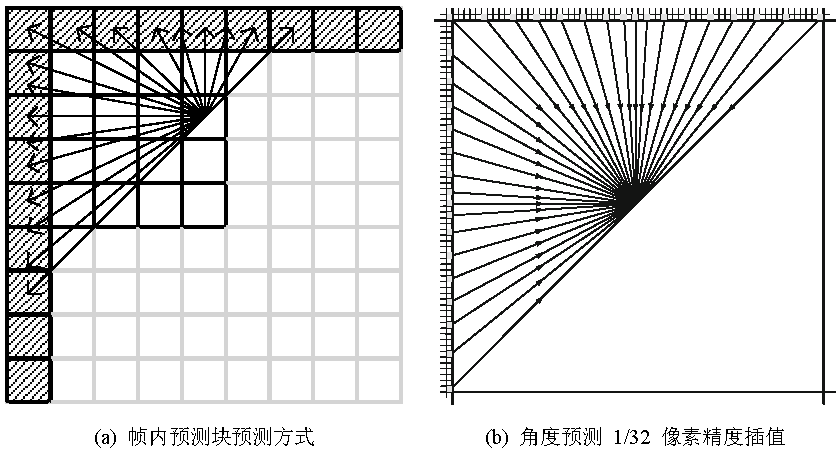
\includegraphics{IntraAngModeOverview.pdf}
    \caption{H.265 帧内预测角度模式}
    \label{fig:IntraAngModeOverview}
\end{figure}
\begin{figure}[hbt]
    \centering
    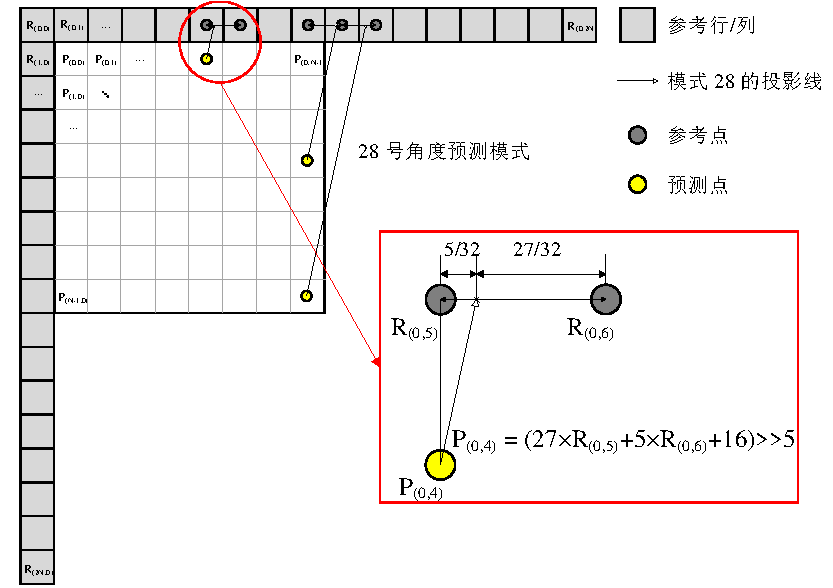
\includegraphics{Projection1_32Precision.pdf}
    \caption{H.265 角度预测 1/32 精度投影}
    \label{fig:Projection1_32Precision}
\end{figure}
显然可选择的方向越多越有可能得到准确的预测值,例如 H.266 中将可选的方向增加到了 65 种。角度预测的过程可以直观地理解为:使用待预测块左侧一列与上侧一行的参考点进行插值与投影。值得一提的是确定投影角度、插值时的权重分配均是以 1/32 像素精度进行的。坐标 $(x,y)$ 处的预测值 $P_{(x,y)}$ 的计算方式如下式:
\begin{equation}
    P_{(x,y)}=((32-\omega)R_{(0,i)}+\omega R_{(0,i+1)}+16)>>5
    \label{equ:IntraProjection}
\end{equation}
其中 $R_{(0,i)}$ 与 $R_{(0,i+1)}$ 表示从待预测点投影到参考行、列时投影点左右的参考点数值,$\omega$ 用于控制权重分配,精度为 1/32,投影点距离 $R_{(0,i+1)}$ 越近 $\omega$ 越大。图 \ref{fig:Projection1_32Precision} 展示了 28 号角度预测模式下的投影与计算。

图 \ref{fig:IntraProjection} 展示了一个 8$\times$8 大小的 PU 经过 H.265 的 35 种帧内预测方式后分别得到的预测结果。参考点取值波动极大,说明该待预测块附近很可能是纹理丰富的区域,因此从不同角度进行投影后得到的预测结果也呈现出丰富的边缘信息。
\begin{figure}[hbt]
    \centering
    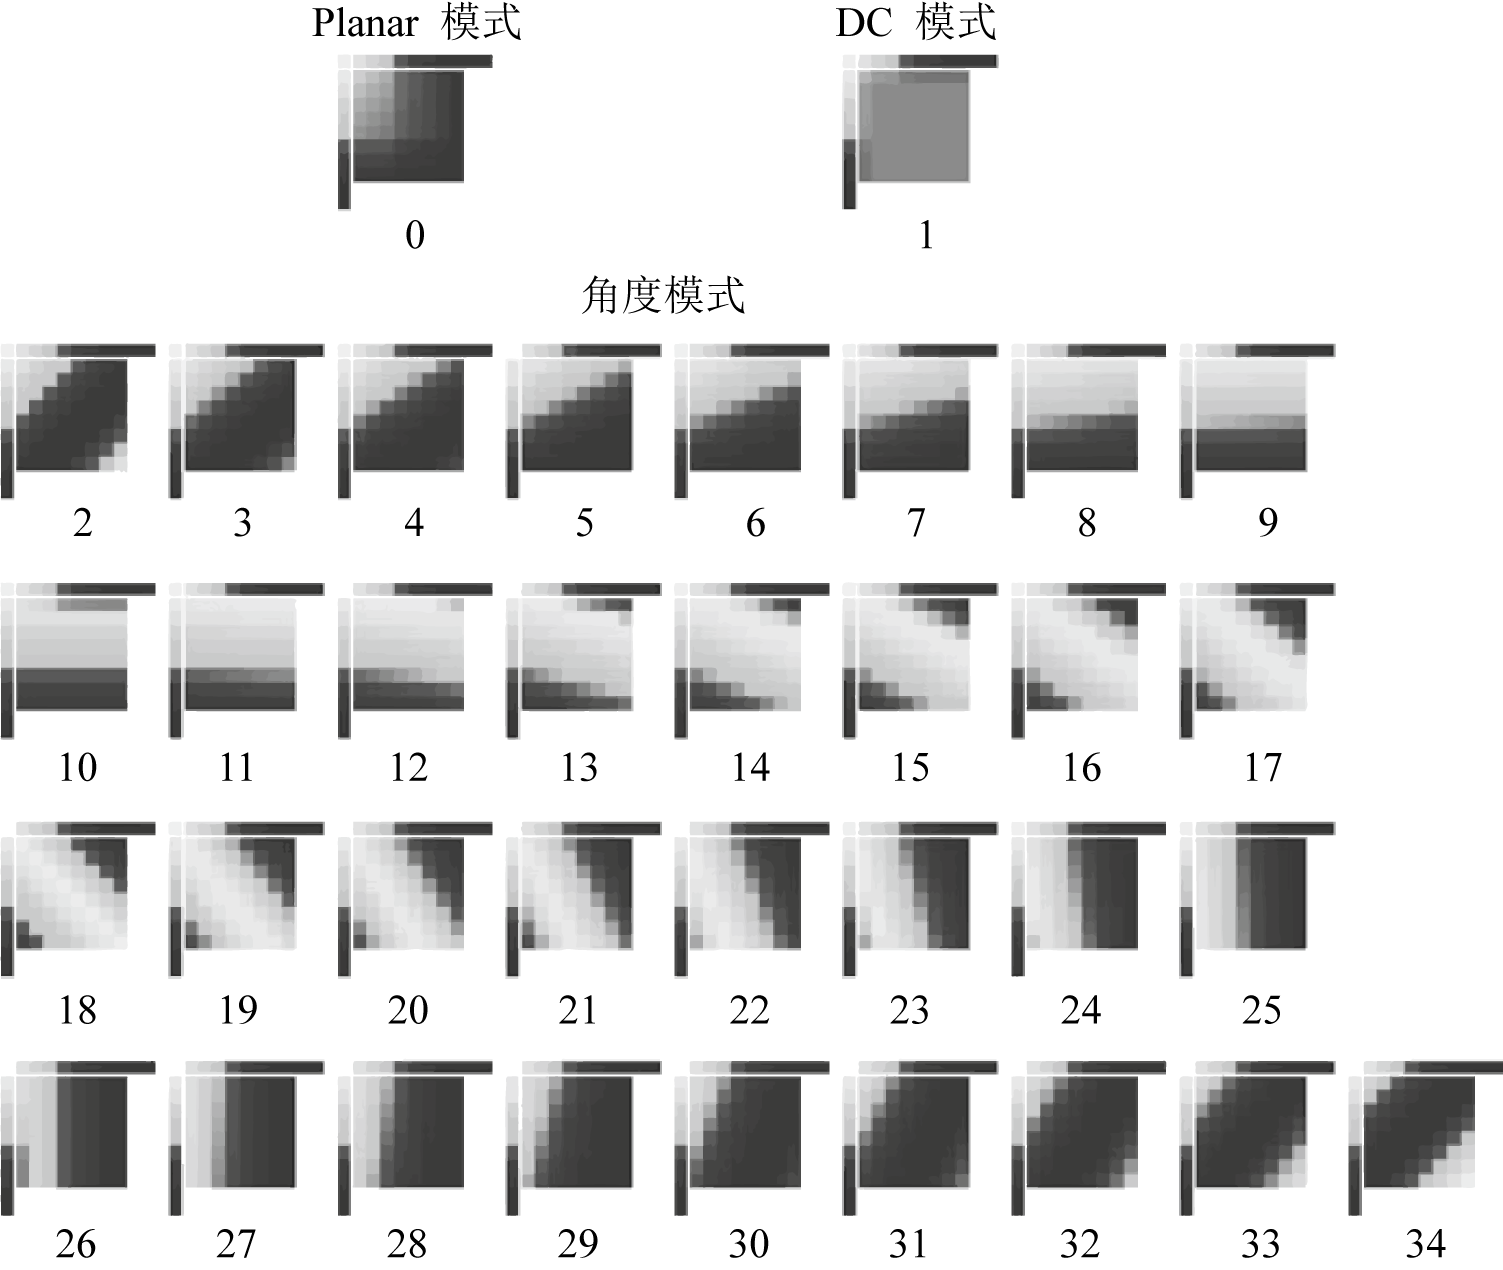
\includegraphics{IntraProjection.png}
    \caption{H.265 帧内预测结果示例}
    \label{fig:IntraProjection}
\end{figure}

最后,帧内预测过程还包含缺失参考点的填补方法、参考点的滤波策略和模式信息的编码方案等重要细节,但与将要提出的优化算法并无直接关系,暂不详述。在充分理解 H.26X 帧内预测的物理意义及预测过程后,下一节将分析其存在的缺陷并提出改进算法。

\subsection{L 形迭代预测算法}
\label{cha:L-IPOverview}
\begin{figure}[hbt]
    \centering
    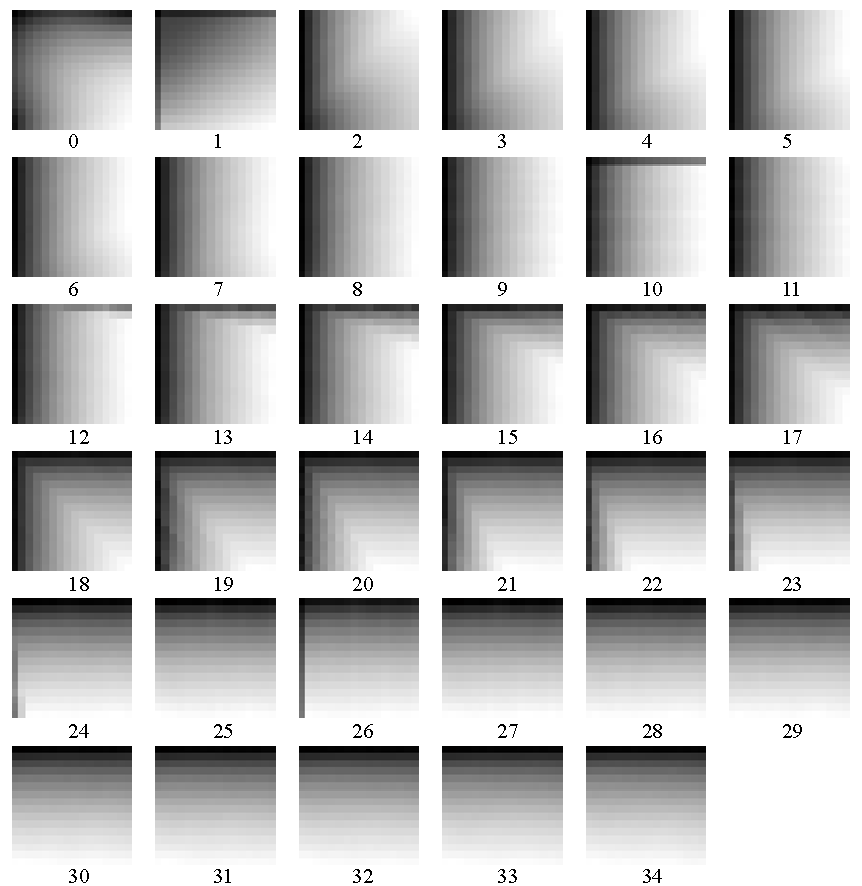
\includegraphics{ResidualVisible.pdf}
    \caption{H.265 帧内预测所有模式残差分布可视图}
    \label{fig:ResidualVisible}
\end{figure}
显然,距离参考行、列越远的待预测点越有可能得到误差大的预测值,这是自然图像朴素的特性决定的。出于研究的严谨性,可通过统计大量预测单元的残差分布来验证这一结论\upcite{ResidualVisible}。图 \ref{fig:ResidualVisible} 是 16$\times$16 大小的预测单元,在所有 35 种帧内预测模式下产生的残差分布可视图,统计的对象来自 JCT-VC 推荐的 H.265 测试序列\upcite{HEVCCommonTestConditionsCTC}中的 Traffic, Kimono, BasketballDrill, FourPeople 4 个序列的第一帧。图中颜色越深表示残差幅值越小即预测准确,反之颜色越淡表示预测越不准确。

分析图 \ref{fig:ResidualVisible} 的残差分布可得 2 条结论:1) 预测值的不准确性随着被预测点与参考点的距离增大而提升。换句话说,靠近参考点的待预测点能被准确地预测,较远区域的待预测点得到的预测效果差。这一现象是空间相关性随着预测距离增大而衰减造成的;2) 不同的预测模式下,靠近参考点的边界区域的预测准确度变化很大。观察图可以发现,模式 2\textasciitilde9 中左侧边界的预测准确度远高于上侧边界,这是由于模式 2\textasciitilde9 的预测过程中用到更多的左侧参考点,这些参考点十分靠近左边界。相反地,模式 27\textasciitilde34 的预测过程中用到更多的上侧参考点,因此表现为上侧边界的预测准确度高。

基于上述分析,为了对抗帧内预测中远离参考点的区域预测效果差的缺陷,本课题提出了 L 形迭代预测算法 L-IP。L-IP 的核心思想是将二维待预测块分割为一系列一维 L 形($\ulcorner$ 形)区域,各 L 形区域自左上角开始迭代地进行帧内预测,每次预测的参考点均为临近的上一次迭代的 L 形区域。对于一个 N$\times$N 大小的预测单元,算法将其分割为 N-1 个 L 形区域和 1 个像素点(处于右下角的像素点),如图 \ref{fig:L-IPOverview}(a) 所示。
第一个 L 形区域 L1 与 H.265 标准的帧内预测一致,使用预测块外的左侧和上侧参考点(L0)进行预测,其余包含 m 个像素点的 L 形区域均使用包含 m+2 个像素点的上一次迭代后的重建区域作为参考点进行预测。除去参考点位置不同,剩余的预测过程几乎与 H.26X 一致,同样使用投影与插值实现预测:
\begin{equation}
    P_{(x,y)}^{L_j} =((32-\omega)R_{(0,i)}^{L_{j-1}} +\omega R_{(0,i+1)}^{L_{j-1}} +16)>>5
    \label{equ:L-IP}
\end{equation}
式中使用上标 $L_j$ 表示样点所处的 L 形区域,其余物理量与式 \ref{equ:IntraProjection} 意义一致。
\begin{figure}[hbt]
    \centering
    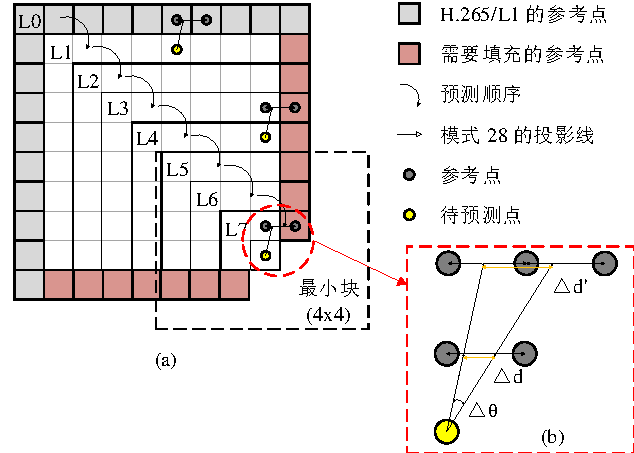
\includegraphics{L-IPOverview.pdf}
    \caption{L-IP 算法}
    \label{fig:L-IPOverview}
\end{figure}

L-IP 算法使待预测点与参考点的距离缩短到了 1 单位,使预测精度大幅上升。同时带来的一个优化是预测过程中不可用的需要填充的参考点(图 \ref{fig:L-IPOverview}(a) 中红色点)更加精确,距离可用点仅 1 单位,而在 H.26X 的块结构预测框架中,一个 N$\times$N 大小的预测单元需要填充的不可用参考点可能距离可用点远达 N 单位。另外,观察图 \ref{fig:Projection1_32Precision} 与图 \ref{fig:L-IPOverview}(b) 可发现在相邻的 2 个角度预测模式间切换时,待预测点(黄色圆点)对应的参考点(灰色圆点)的权重分配会根据 $\Delta d$ 产生变化,当待预测点远离参考点时,相邻 2 个角度模式的切换将产生较大的 $\Delta d{'}$ 致使权重分配变得十分粗犷,不利于在纹理丰富的区域生成变化精细的预测值。在 L-IP 算法方案中,这个缺陷由于待预测点与参考点的距离缩短到 1 单位而不再存在。

L-IP 算法中有 2 个细节需要说明:
1) 尽管我们可以严格地按照式 \ref{equ:L-IP} 从 L1 迭代预测到右下角的最后一个像素点,但我们在测试过程中发现,L-IP 算法需要对预测单元内的每一个 L 区域记录一个预测模式信息,在 L 形区域足够小的情况下,提高极少量待预测点的预测准确度带来的收益甚至无法抵消记录额外模式信息的开销。经过大量的实验统计,我们将 4$\times$4 大小的待预测块规定为最小块,以图 \ref{fig:L-IPOverview} 为例,L1\textasciitilde L4 应用 L-IP 算法,右下角的 4$\times$4 块则应用 H.26X 的基于块结构的预测;
2) 由于需要对每个 L 形区域记录一个预测模式信息,使用 6bits 的码字编码 35 种预测模式之一显得代价过大,又因为待预测点与参考点的距离缩短,使并不需要如此密集的角度模式。基于上述 2 点原因,L-IP 中每个 L 形区域仅在 8 个预测模式中进行选择,一方面减少了模式信息的数据量,另一方面一定程度上加快了编码速度。
另外,应用了 L-IP 算法并非完全舍弃 H.26X 基于块结构的预测。对于每个 PU,均分别应用 L-IP 算法预测和基于块结构的预测,选择率-失真代价较小的一方,换句话说,L-IP 与 H.26X 原始算法共同加入了编码的 RDO 过程。

\subsection{算法性能测试与分析}
\label{cha:L-IPTest}
L-IP 提出的初衷是提高远距离待预测点的预测准确度,为了验证预测准确度的改进,对 H.265 基于块结构的预测残差和 L-IP 算法得到的预测残差进行统计。统计的对象来自 JCT-VC 推荐的 H.265 测试序列中的 BasketballDrive(ClassB), Kimono(ClassB), PartyScene(ClassC), Johnny(ClassE), SlideEditing(ClassF)。统计结果如表 \ref{tab:L-IPResidualReduction} 所示。
统计结果显示,在 4$\times$4 大小的预测单元中预测残差的平均幅值降低了 20.43\%,在 8$\times$8 PU 中这一数值是 22.14\%,在 16$\times$16 PU 中是 31.36\%,由于 32$\times$32 大小的 PU 数量过少,不具有统计意义,不在表中列出。
\begin{table}[hbt]
    \centering
    \caption{H.265 与 L-IP 各尺寸 PU 平均残差幅值统计}
    \label{tab:L-IPResidualReduction}
    \begin{tabular}{@{}clcccccc@{}}
        \toprule
        \multirow{2}{*}{序列类别}                & \multicolumn{1}{c}{\multirow{2}{*}{序列}} & \multicolumn{2}{c}{4$\times$4 PU} & \multicolumn{2}{c}{8$\times$8 PU} & \multicolumn{2}{c}{16$\times$16 PU}                             \\ \cmidrule(l){3-8}
                                                 & \multicolumn{1}{c}{}                      & H.265                             & L-IP                              & H.265                               & L-IP   & H.265   & L-IP   \\ \midrule
        \multirow{2}{*}{ClassB}                  & BasketballDrive                           & 30.01                             & 26.54                             & 130.94                              & 116.08 & 536.56  & 401.07 \\
                                                 & Kimono                                    & 27.39                             & 20.58                             & 100.63                              & 86.52  & 371.53  & 291.05 \\
        ClassC                                   & PartyScene                                & 109.97                            & 98.62                             & 463.98                              & 316.04 & 1067.07 & 860.59 \\
        ClassE                                   & Johnny                                    & 27.85                             & 17.23                             & 82.54                               & 60.19  & 230.74  & 164.25 \\
        ClassF                                   & SlideEditing                              & 163.6                             & 135.32                            & 337.67                              & 248.71 & 1464.68 & 560.35 \\ \midrule
        \multicolumn{2}{l}{残差平均幅值降低比率} & \multicolumn{2}{c}{20.43\%}               & \multicolumn{2}{c}{22.14\%}       & \multicolumn{2}{c}{31.36\%}                                                                         \\ \bottomrule
    \end{tabular}
\end{table}

H.26X 传统的基于块结构的预测中,每个预测单元仅使用 1 种预测模式,这使得图像中纹理丰富的区域必定被划分为多而小的预测单元。L-IP 算法下,大尺寸预测单元的每个 L 形区域均有一个独立的预测模式,因此应用 L-IP 后将使得 PU 划分结果中出现更多的大尺寸 PU。这一结论亦被实验数据验证,如表 \ref{tab:L-IPPUSize} 所示。表中数据的含义是:一帧中有 x\% 的像素点是在 N$\times$N 大小的预测单元中进行预测得到的。根据统计结果,16$\times$16 与 32$\times$32 的大尺寸预测单元分别增加了 18.67\% 和 33.04\%,4$\times$4 与 8$\times$8 的小尺寸预测单元则分别减少了 47.42\% 和 4.29\%。
\begin{table}[hbt]
    \centering
    \caption{H.265 与 L-IP 各尺寸 PU 占比统计}
    \label{tab:L-IPPUSize}
    \begin{tabular}{@{}lcccccccc@{}}
        \toprule
        \multicolumn{1}{c}{\multirow{2}{*}{序列}} &
        \multicolumn{2}{c}{4$\times$4 PU/\%}      &
        \multicolumn{2}{c}{8$\times$8 PU/\%}      &
        \multicolumn{2}{c}{16$\times$16 PU/\%}    &
        \multicolumn{2}{c}{32$\times$32 PU/\%}                                                                    \\ \cmidrule(l){2-9}
        \multicolumn{1}{c}{}                      & L-IP  & H.265 & L-IP  & H.265 & L-IP  & H.265 & L-IP  & H.265 \\ \midrule
        PeopleOnStreet                            & 19.27 & 90.24 & 5.58  & 8.24  & 28.21 & 1.45  & 46.94 & 0.07  \\
        Traffic                                   & 14.93 & 87.80 & 4.22  & 11.46 & 29.50 & 0.70  & 51.35 & 0.05  \\
        BasketballDrive                           & 48.44 & 63.73 & 22.78 & 26.49 & 16.30 & 9.36  & 12.48 & 0.43  \\
        BQTerrace                                 & 42.09 & 72.62 & 11.98 & 15.54 & 19.79 & 7.61  & 26.14 & 4.22  \\ \midrule
        \multicolumn{1}{c}{PU 数量变化率}         &
        \multicolumn{2}{c}{-47.42}                &
        \multicolumn{2}{c}{-4.29}                 &
        \multicolumn{2}{c}{18.67}                 &
        \multicolumn{2}{c}{33.04}                                                                                 \\ \bottomrule
    \end{tabular}
\end{table}

最后,应用 L-IP 算法进行实际编码测试,与 H.265 标准参考软件 HM-16.21\upcite{HEVCsoftwareHM16} 编码结果对比,统计出编码效率提升的幅度。测试的对象为 JCT-VC 推荐的标准测试序列,包括 5 类自然图像:ClassA(2560$\times$1600), ClassB(1080p), ClassC(WVGA), ClassD(WQVGA), ClassE(720p) 和 1 类屏幕图像:ClassF。测试严格按照 H.265 通用测试环境 (Common Test Condition, CTC)\upcite{HEVCCommonTestConditionsCTC}进行配置,由于所提 L-IP 算法是为帧内无损编码设计的,因此仅在全帧内 (All Intra, AI) 的无损配置下进行测试。统计结果如表 \ref{tab:L-IPSummary} 所示。

使用码率降低的百分比来衡量算法性能,表中负值表示使用 L-IP 算法编码得到的结果码率对比 H.265 标准降低。使用编码时间衡量算法复杂度,表中的编码时间、解码时间百分比数值由下式计算得到:
\begin{equation}
    \Delta T=\frac{T_{proposed}}{T_{anchor}}\times 100\%
\end{equation}
$T_{proposed}$ 表示所提算法的编码或解码所用时间,$T_{anchor}$ 表示 HM 参考软件编码或解码用时。ClassA\textasciitilde E 中,序列 FourPeople 得到了最大的 12.51\% 的编码效率提升,均值为 8.10\%;ClassF 中,序列 SlideShow 获得了最大的 22.26\% 的编码效率提升,均值为 14.76\%。算法复杂度方面,L-IP 使编码时间增加了 25\%,解码时间基本不变,证明 L-IP 算法性能良好,具有较高的应用价值。
\begin{table}[!p]
    \centering
    \caption{L-IP 算法性能测试}
    \label{tab:L-IPSummary}
    \begin{tabular}{@{}clccc@{}}
        \toprule
        序列类别                               & \multicolumn{1}{c}{序列}     & 分辨率           & 码率     & 编码时间 \\ \midrule
        \multirow{2}{*}{ClassA}                & PeopleOnStreet               & 2560$\times$1600 & -11.29\% & 125.98\% \\
                                               & Traffic                      & 2560$\times$1600 & -11.46\% & 124.76\% \\
        \multirow{5}{*}{ClassB}                & BasketballDrive              & 1920$\times$1080 & -4.20\%  & 126.57\% \\
                                               & BQTerrace                    & 1920$\times$1080 & -8.57\%  & 125.85\% \\
                                               & Cactus                       & 1920$\times$1080 & -3.74\%  & 126.96\% \\
                                               & Kimono                       & 1920$\times$1080 & -7.71\%  & 127.41\% \\
                                               & ParkScene                    & 832$\times$480   & -6.58\%  & 127.37\% \\
        \multirow{4}{*}{ClassC}                & BasketballDrill              & 832$\times$480   & -5.51\%  & 126.32\% \\
                                               & BQMall                       & 832$\times$480   & -6.17\%  & 126.48\% \\
                                               & PartyScene                   & 832$\times$480   & -5.58\%  & 125.11\% \\
                                               & RaceHorsesC                  & 832$\times$480   & -8.10\%  & 124.38\% \\
        \multirow{4}{*}{ClassD}                & BasketballPass               & 416$\times$240   & -12.36\% & 124.54\% \\
                                               & BlowingBubbles               & 416$\times$240   & -5.47\%  & 125.01\% \\
                                               & BQSquare                     & 416$\times$240   & -5.27\%  & 124.80\% \\
                                               & RaceHorses                   & 416$\times$240   & -8.51\%  & 125.34\% \\
        \multirow{3}{*}{ClassE}                & FourPeople                   & 1280$\times$720  & -12.51\% & 124.64\% \\
                                               & Johnny                       & 1280$\times$720  & -10.97\% & 124.51\% \\
                                               & KristenAndSara               & 1280$\times$720  & -11.86\% & 123.96\% \\
        \multirow{4}{*}{ClassF}                & BasketballDrillText          & 832$\times$480   & -6.07\%  & 124.67\% \\
                                               & ChinaSpeed                   & 1024$\times$768  & -17.15\% & 121.53\% \\
                                               & SlideEditing                 & 1280$\times$720  & -13.57\% & 123.07\% \\
                                               & SlideShow                    & 1280$\times$720  & -22.26\% & 126.19\% \\ \midrule
        \multicolumn{2}{l}{ClassA$\sim$E 均值} & -                            & -8.10\%          & 125.56\%            \\ \midrule
        \multicolumn{2}{l}{ClassF 均值}        & -                            & -14.76\%         & 123.87\%            \\ \midrule
        \multicolumn{2}{l}{ClassA$\sim$F 均值} & -                            & -9.31\%          & 125.25\%            \\ \midrule
        \multicolumn{2}{l}{解码时间}           & \multicolumn{3}{c}{103.21\%}                                          \\ \bottomrule
    \end{tabular}
\end{table}

\section{帧内无损编码的分块过程优化}
\label{cha:L-BPSec}
H.26X 的帧内分块方案中,基于四叉树结构的分块算法决定了一个预测单元仅可在保留 2N$\times$2N 结构与划分为 4 个 N$\times$N 结构这 2 个选项中进行选择。尽管这能有效地做到在不同纹理丰富程度的区域自适应选择分块大小,但过于粗暴的 2 选 1 导致每划分一次 N$\times$N 结构都产生 4 组需要独立编码的模式信息、分块信息及其他辅助信息,一定程度上降低了编码效率。本节将针对该缺陷进行分析与优化。

\subsection{帧内分块决策过程分析}
H.265 标准将 H.264 中 16$\times$16 的宏块扩展到了 64$\times$64,并且使用编码树单元 (Coding Tree Unit, CTU) 和 CU 取代了 H.264 中宏块的概念,同时应用基于四叉树的分块方案使分块的大小根据图像中纹理丰富与否进行自适应调整。例如,在图像中平滑或仅含简单纹理的区域,以大块的形式进行预测和编码,节省了大量预测模式与分块模式信息的开销,从而提高编码效率,但也一定程度上降低了预测的准确性。而在纹理丰富的区域将大块划分为大量小尺寸的预测块,使预测残差减小,但同时会产生大量需要额外编码的模式信息和分块标志信息。因此,我们需要在预测准确性和编码产生的数据量之间寻找折衷,这也是 H.265 中 RDO 的重要一环。HM 参考软件中的 RD 代价 $J_{mode}$ 计算方式如式 \ref{equ:RDcost}。
\begin{equation}
    J_{mode}=B_{mode}+\lambda_{mode}\cdot SSE
    \label{equ:RDcost}
\end{equation}
其中 $B_{mode}$ 表示编码当前单元产生的数据量,重建块的误差平方和 $SSE$ 用于衡量失真,有时也用绝对误差和或 PSNR 进行衡量,$\lambda_{mode}$ 为拉格朗日因子。在无损编码中重建块不再存在失真,RD 代价的计算简化为:
\begin{equation}
    J_{mode}=B_{mode}
\end{equation}
在编码过程中,RDO 用于搜寻最佳的预测模式与最佳的分块模式。

编码时,一帧图像首先被切分为若干大小相等的 CTU,RDO 将从最小的 4$\times$4 分块开始向上搜索,以 RD 代价为依据确定最终一个 CTU 的分块模式。
图 \ref{fig:PartitionExample}(a) 展示了一个 CTU 的分块结果,每个方框代表一个独立的预测单元,对于每一个单元都将编码 1 个分块标志指示当前块是否往下切分一次。
\begin{figure}[hbt]
    \centering
    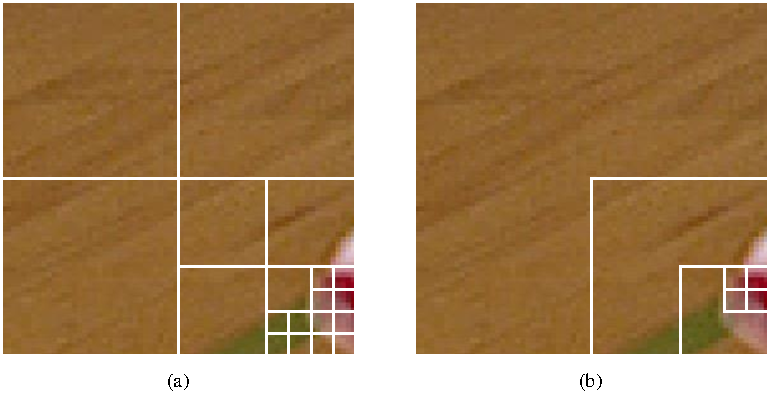
\includegraphics{PartitionExample.pdf}
    \caption{基于四叉树的分块算法与 L-BP 算法}
    \label{fig:PartitionExample}
\end{figure}
从图中可观察到在基于四叉树结构的分块算法下,由于右下角区域存在极小部分纹理丰富的区域,CTU 经过 RDO 被切分为 19 个独立进行预测的小块,因此编码该 CTU 需要处理的数据有:64$\times$64 个预测残差;19 个预测模式信息;13 个分块标志。尽管左、上侧 3 个较大块可能使用的是相同的预测模式,也必须编码 3 次预测模式信息,一定程度上降低了编码效率。在充分理解 H.26X 帧内分块过程存在的缺陷后,下一节将提出本课题的改进算法。

\subsection{L 形分块算法}
根据上节所分析,在 H.265 传统的基于四叉树结构的分块算法下,一旦当前 2N$\times$2N 大小的编码单元存在小区域的丰富纹理,该单元大概率将根据 RD 代价判断切分为 4 个 N$\times$N 大小的子单元分别进行预测和编码,从而增加了 3 个需要额外编码的预测模式信息。并且,如果应用了 \ref{cha:L-IPOverview} 节所述的 L-IP 算法,一个 N$\times$N 大小的预测单元需要记录 N-3 个预测模式信息,需要额外编码的预测模式将进一步增加。考虑到这一情况,结合 L-IP 的预测结构,本课题提出了一种 L 形分块算法 L-BP。L-BP 可以保证编码单元仅包含小区域丰富纹理时,使编码单元仍保持大块的结构进行预测和编码,以减少预测模式信息的增加量,最大化 L-IP 算法带来的增益。

L-BP 算法的核心思想是将一个需要向下切分的编码单元视为 2 部分组成:一个 L 形区域和一个块状区域,而非四叉树结构下大小均等的 4 部分。其中 L 形区域是由四叉树结构下的 3 个块状区域组合而成,根据 3 个块状不同位置的组合,将产生 4 种可能性:$\ulcorner \llcorner \urcorner \lrcorner$,图 \ref{fig:PartitionExample}(b) 展示了 L-BP 的分块结果,其中出现了两种 L 形分块模式($\ulcorner \llcorner$)。对于剩下的块状区域,将继续判断是否进行 L-BP 分块,直到分割到最小单元。整体的分块决策流程与 H.265 一致,从底层向上搜索。值得一提的是提出 L-BP 算法的同时并未抛弃 H.265 基于四叉树的分块算法,换句话说,L-BP 提供了 4 种新的可能的分块模式,分块决策时从 H.265 的 2 选 1 增加到了 6 选 1,使分块更加灵活,以适应不同纹理丰富程度的区域。

图 \ref{fig:L-BP}(a)(b) 对比了一个 CTU 在 H.265 基于四叉树结构的分块算法和加入了 L-BP 算法后的分块结果。图 \ref{fig:L-BP}(c) 展示了加入了 L-BP 算法后的整体分块决策流程,在每一个层级均提供了 6 个分块模式进行选择。
\begin{figure}[!p]
    \begin{adjustbox}
        {
            addcode=
                {\begin{minipage}{\width}}
                        {
                        \caption{应用 L-BP 算法后的分块决策流程}
                        \label{fig:L-BP}
                    \end{minipage}
                }
            ,rotate=90,center
        }
        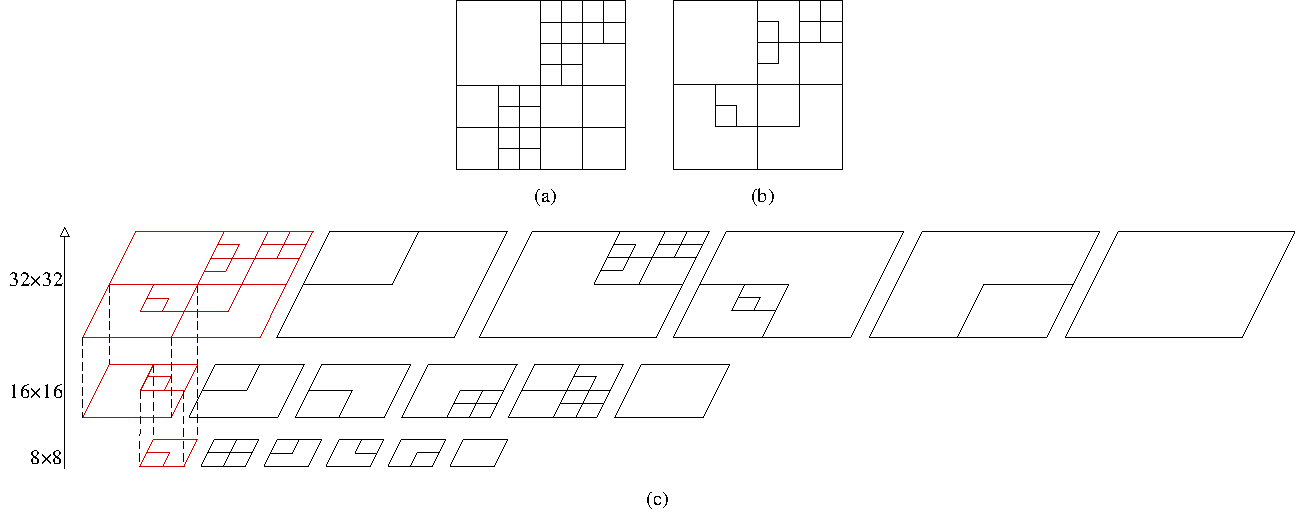
\includegraphics{L-BP.pdf}
    \end{adjustbox}
\end{figure}

\subsection{算法性能测试与分析}
\label{cha:L-BPTest}
最后,应用 L-BP 算法进行实际编码测试,与 H.265 标准参考软件 HM-16.21\upcite{HEVCsoftwareHM16} 编码结果对比,统计出编码效率提升的幅度。测试的对象和环境与 \ref{cha:L-IPTest} 节所述相同,不再赘述。统计结果如表 \ref{tab:L-BPSummary} 所示。

使用码率降低的百分比来衡量算法性能,表中负值表示使用 L-BP 算法编码得到的结果码率对比 H.265 标准降低。
ClassA\textasciitilde E 中,序列 KristenAndSara 得到了最大的 4.40\% 的编码效率提升,均值为 2.04\%;ClassF 中,序列 SlideShow 获得了最大的 5.43\% 的编码效率提升,均值为 3.70\%。
使用编码时间衡量算法复杂度,L-BP 算法几乎没有影响编码、解码时间。统计数据证明 L-BP 算法性能良好,具有较高的应用价值。

\begin{table}[!p]
    \centering
    \caption{L-BP 算法性能测试}
    \label{tab:L-BPSummary}
    \begin{tabular}{clccc}
        \toprule
        序列类别                               & \multicolumn{1}{c}{序列}     & 分辨率           & 码率     & 编码时间 \\ \midrule
        \multirow{2}{*}{ClassA}                & PeopleOnStreet               & 2560$\times$1600 & -1.78\%  & 100.98\% \\
                                               & Traffic                      & 2560$\times$1600 & -1.89\%  & 100.03\% \\
        \multirow{5}{*}{ClassB}                & BasketballDrive              & 1920$\times$1080 & -2.28\%  & 101.06\% \\
                                               & BQTerrace                    & 1920$\times$1080 & -1.80\%  & 101.31\% \\
                                               & Cactus                       & 1920$\times$1080 & -1.15\%  & 101.28\% \\
                                               & Kimono                       & 1920$\times$1080 & -1.57\%  & 101.27\% \\
                                               & ParkScene                    & 832$\times$480   & -1.48\%  & 101.29\% \\
        \multirow{4}{*}{ClassC}                & BasketballDrill              & 832$\times$480   & -1.96\%  & 100.82\% \\
                                               & BQMall                       & 832$\times$480   & -1.46\%  & 100.82\% \\
                                               & PartyScene                   & 832$\times$480   & -1.42\%  & 100.49\% \\
                                               & RaceHorsesC                  & 832$\times$480   & -1.46\%  & 100.50\% \\
        \multirow{4}{*}{ClassD}                & BasketballPass               & 416$\times$240   & -2.62\%  & 100.00\% \\
                                               & BlowingBubbles               & 416$\times$240   & -1.05\%  & 100.00\% \\
                                               & BQSquare                     & 416$\times$240   & -1.54\%  & 100.63\% \\
                                               & RaceHorses                   & 416$\times$240   & -1.17\%  & 101.32\% \\
        \multirow{3}{*}{ClassE}                & FourPeople                   & 1280$\times$720  & -3.52\%  & 100.73\% \\
                                               & Johnny                       & 1280$\times$720  & -4.11\%  & 100.95\% \\
                                               & KristenAndSara               & 1280$\times$720  & -4.40\%  & 100.80\% \\
        \multirow{4}{*}{ClassF}                & BasketballDrillText          & 832$\times$480   & -1.96\%  & 101.00\% \\
                                               & ChinaSpeed                   & 1024$\times$768  & -4.75\%  & 100.45\% \\
                                               & SlideEditing                 & 1280$\times$720  & -2.64\%  & 100.66\% \\
                                               & SlideShow                    & 1280$\times$720  & -5.43\%  & 102.68\% \\ \midrule
        \multicolumn{2}{l}{ClassA$\sim$E 均值} & -                            & -2.04\%          & 100.79\%            \\ \midrule
        \multicolumn{2}{l}{ClassF 均值}        & -                            & -3.70\%          & 101.20\%            \\ \midrule
        \multicolumn{2}{l}{ClassA$\sim$F 均值} & -                            & -2.34\%          & 100.87\%            \\ \midrule
        \multicolumn{2}{l}{解码时间}           & \multicolumn{3}{c}{100.71\%}                                          \\ \bottomrule
    \end{tabular}
\end{table}

\section{帧内无损编码的待编码系数再处理}
H.26X 系列标准可以通过简单地跳过变换、量化、去块滤波、自适应样点补偿等可能引入失真的步骤,实现帧内无损压缩。但也因此使得待编码系数具有较高的能量,为后续的熵编码带来了极大的压力。
本节将针对该缺陷进行分析与优化。

\subsection{帧内预测残差分析}
无损编码方案中跳过了量化步骤,此时待编码数据不再是变换域系数而是预测残差,因此其仍具有空间域的物理意义。为了直观地验证这一结论,尝试将残差绘制出来观察。图 \ref{fig:ResidualImage} 展示了在H.265标准下经过帧内预测后的残差图像(数值整体平移了128以绘制负值)。
\begin{figure}[hbt]
    \centering
    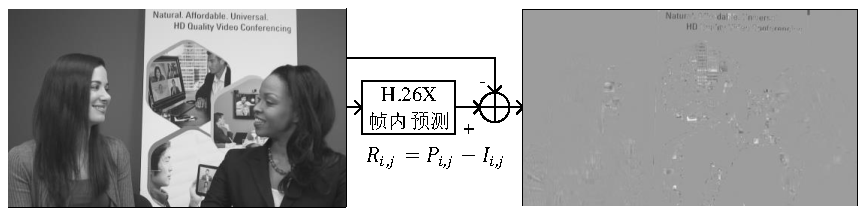
\includegraphics{ResidualImage.pdf}
    \caption{KristenAndSara 第一帧及其帧内预测残差(亮度)}
    \label{fig:ResidualImage}
\end{figure}

出于多种原因,尽管帧内预测的准确性不断提高(H.264 仅使用 9 种预测模式,H.265 增加到 35 种,H.266 达到了 67 种),残差中仍然可能保留丰富的边缘特征。首先,由于 PU 最小尺寸的限制,角度预测在图像中纹理丰富的区域始终无法得到良好的预测结果;其次,当被预测块靠近参考像素的边沿存在不连续性时,角度预测很可能会插入原始块中本不存在的方向性条纹。

帧内预测的目的是消除图像的空间相关性,显然,通过帧内预测得到的残差仍具有较强的特殊的空间相关性。与自然图像不同,帧内预测残差的空间相关性体现为含有丰富的边缘特征。在充分理解 H.26X 帧内预测残差存在的特征后,下一节将提出本课题的改进算法。

\subsection{残差中值边缘检测算法}
为了利用帧内预测残差特殊的空间相关性,进一步提高视频帧内编码的效率,本课题提出了一种在 H.264、H.265、H.266 中通用的基于残差中值边缘检测的待编码系数再处理算法 R-MED。R-MED 利用了帧内预测残差具有丰富的边缘特征这一统计结果,对预测残差进行二次预测。首先将当前编码块的残差首行、首列作为参考点;然后利用中值边缘检测对剩余点逐点进行预测并求得新的残差;最后统计处理前后的残差能量,选择能量较小的一组进行熵编码。如图 \ref{fig:RMEDOverview}(c) 所示。
\begin{figure}[hbt]
    \centering
    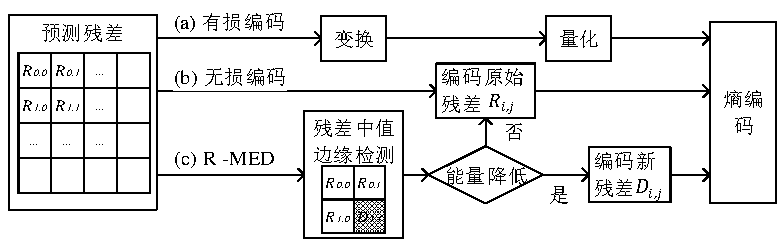
\includegraphics{RMEDOverview.pdf}
    \caption{H.26X 无损编码方案及 R-MED 应用方案}
    \label{fig:RMEDOverview}
\end{figure}

中值边缘检测 MED 已被应用在图像的低复杂度无损压缩 (Low Complexity Lossless Compression for Images, LOCO-I)\upcite{LOCO-i} 算法中。但与 LOCO-I 使用 MED 对原始像素进行预测不同,考虑到 MED 具有很强的边缘检测能力,恰好残差图像中包含丰富的边缘特征,因此将其应用到残差图像的二次预测上。R-MED 的新预测值 $P_{i,j}^{'}$ 由下式给出:
\begin{equation}
    P_{i,j}^{'}=\left\{
    \begin{aligned}
        \min(R_{i,j-1},R_{i-1,j}), \quad       & R_{i-1,j-1} \geqslant \max(R_{i,j-1},R_{i-1,j}) \\
        \max(R_{i,j-1},R_{i-1,j}), \quad       & R_{i-1,j-1} \leqslant \min(R_{i,j-1},R_{i-1,j}) \\
        R_{i,j-1}+R_{i-1,j}-R_{i-1,j-1}, \quad & o.w
    \end{aligned}
    \right.
    \label{equ:LOCO-i}
\end{equation}
式中 $R_{i,j}$ 表示 H.26X 经过帧内预测后得到的残差。如图 \ref{fig:RMEDcalculate} 所示,R-MED 可以精准地得到强边缘处的预测值。
当 $R_{i-1,j-1} \geqslant \max(R_{i,j-1},R_{i-1,j})$ 时(见图 \ref{fig:RMEDcalculate}(a)),如果 $R_{i,j-1}>R_{i-1,j}$,那么在 $P_{i,j}^{'}$ 左侧的垂直方向上很可能存在明显的垂直边缘,此时最佳预测值为 $R_{i-1,j}$;反之则很可能在上方存在明显的水平边缘,此时最佳预测值为 $R_{i,j-1}$。类似地,图 \ref{fig:RMEDcalculate}(b) 展示了 $R_{i-1,j-1} \leqslant \min(R_{i,j-1},R_{i-1,j})$ 时,$P_{i,j}^{'}$ 的选择策略。
\begin{figure}[hbt]
    \centering
    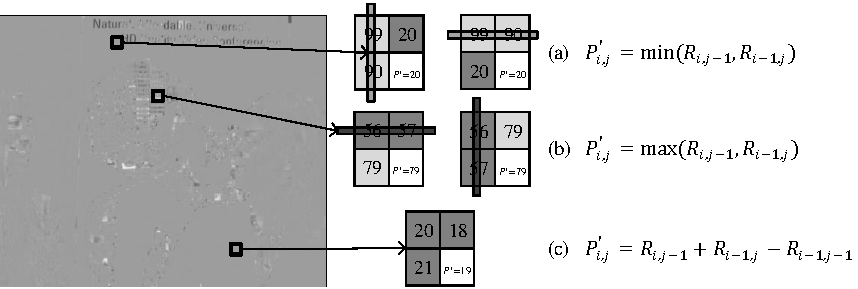
\includegraphics{RMEDcalculate.pdf}
    \caption{R-MED 的预测策略}
    \label{fig:RMEDcalculate}
\end{figure}

此外,如果 R-MED 没有检测到明显的水平或垂直边缘,将采取模仿水平/垂直方向相邻点变化趋势的预测策略。如图 \ref{fig:RMEDcalculate}(c) 所示,$P_{i,j}^{'}$ 周围的参考点并不满足式 \ref{equ:LOCO-i} 的前两个条件,表明该区域变化平坦没有复杂纹理。$P_{i,j}^{'}$ 上方参考点的数值由 20 降低到 18(-2),左侧参考点的数值由 20 增加到 21(+1),因此 $P_{i,j}^{'}$ 模仿上方的变化趋势得到 $P_{i,j}^{'}=R_{i,j-1}-2=21-2=19$,或模仿左侧的变化趋势得到 $P_{i,j}^{'}=R_{i-1,j}+1=18+1=19$。

通过上述分析,证明了 R-MED 具有对边缘信息预测准确的特点,因此适合将其应用到 H.26X 残差图像的二次预测中。R-MED 对经过 H.26X 帧内预测后,进行熵编码前的预测残差进行再处理。以 PU 为基本单位,将各 PU 的首行、首列作为参考点,对剩下的数据点逐点应用 R-MED 算法计算新的残差 $D_{i,j}$:
\begin{equation}
    D_{i,j}=\left\{
    \begin{aligned}
        R_{i,j}, \quad             & i=0 \ \ or \ \ j=0 \\
        P_{i,j}^{'}-R_{i,j}, \quad & o.w
    \end{aligned}
    \right.
\end{equation}
式中 $R_{i,j}$ 表示 H.26X 经过帧内预测后得到的残差,$P_{i,j}^{'}$ 表示通过 R-MED 算法得到的预测值。然后分别计算处理前后的残差总能量 $E_{src}$、$E_{R-MED}$:
\begin{equation}
    E_{src}=\sum_{i=0}^{N-1} \sum_{j=0}^{N-1} R_{i,j}^{2}
\end{equation}
\begin{equation}
    E_{R-MED}=\sum_{i=0}^{N-1} \sum_{j=0}^{N-1} D_{i,j}^{2}
\end{equation}
最后选择总能量较小的一组进行熵编码。通过残差的总能量判断是否选用经过二次处理的残差是因为,H.26X 在对预测残差进行编码前,需要使用哥伦布-莱斯码或指数哥伦布码对其进行二值化,二值化后码字的长度将与残差的绝对幅值呈指数关系\upcite{CoefficientScanBinGolombRice}。图 \ref{fig:RMEDExample} 是一个 4$\times$4 的预测单元经过 H.265+R-MED 算法处理前后的效果,其残差总能量明显降低。
\begin{figure}[hbt]
    \centering
    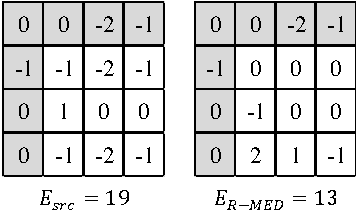
\includegraphics{RMEDExample.pdf}
    \caption{一个经过 R-MED 处理的预测单元}
    \label{fig:RMEDExample}
\end{figure}

\subsection{算法性能测试与分析}
R-MED 算法提出的初衷是充分利用待编码系数的特殊空域相关性,通过再预测降低其整体能量,为了验证降低帧内预测残差能量的效果,统计了在 H.265 标准下,部分测试序列第一帧经过 R-MED 算法处理前后整体能量的变化率。统计结果如表 \ref{tab:RMEDEnergy} 所示,单帧图像的残差能量平均降低了 67.86\%,且表现出高分辨率下性能较好的趋势。
\begin{table}[]
    \centering
    \caption{应用 H.265+R-MED 算法后残差能量的变化率}
    \label{tab:RMEDEnergy}
    \begin{tabular}{@{}clcccc@{}}
        \toprule
        类别 & \multicolumn{1}{c}{序列} & 分辨率           & $\sum_{\rm CU}E_{src}$ & $\sum_{\rm CU}E_{R-MED}$ & 变化率   \\ \midrule
        A    & PeopleOnStreet           & 2560$\times$1600 & 633451646              & 94108069                 & -85.14\% \\
        B    & Kimono                   & 1920$\times$1080 & 73752438               & 11522730                 & -84.38\% \\
        C    & BQMall                   & 832$\times$480   & 59358254               & 25243957                 & -57.47\% \\
        D    & BlowingBubbles           & 416$\times$240   & 14714641               & 8036874                  & -45.38\% \\
        E    & KristenAndSara           & 1280$\times$720  & 97320940               & 12361610                 & -87.30\% \\
        F    & SlideEditing             & 1280$\times$720  & 1133005976             & 595102758                & -47.48\% \\ \midrule
        均值 & \multicolumn{1}{c}{-}    & -                & -                      & -                        & -67.86\% \\ \bottomrule
    \end{tabular}
\end{table}
通过绘制残差图像也能验证 R-MED 降低预测残差空域冗余和整体能量的效果。图 \ref{fig:RMEDResidualImage} 是测试序列 KristenAndSara 第一帧经过 R-MED 处理前后的残差图像,可直观地观察到其边缘特征极大地减少,证明 R-MED 算法对预测残差图像有优秀的处理能力。
\begin{figure}[hbt]
    \centering
    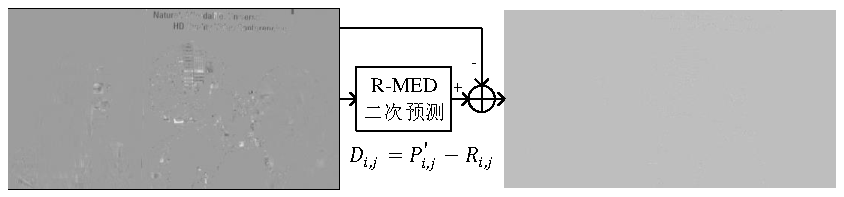
\includegraphics{RMEDResidualImage.pdf}
    \caption{KristenAndSara 第一帧残差经 R-MED 处理后效果(亮度)}
    \label{fig:RMEDResidualImage}
\end{figure}

最后,应用 R-MED 算法进行实际编码测试。与 \ref{cha:L-IPTest} 节、\ref{cha:L-BPTest} 节的测试不同,由于 R-MED 算法通用性极强,可在 H.26X 系列编码标准中通用,因此 R-MED 分别在 H.265 标准参考软件 HM-16.21 和 H.266 标准参考软件 VTM-12.3 中实现,并严格按照 H.265 通用测试环境、H.266 无损编码通用测试环境\upcite{VVCTestConditions},使用 JCT-VC 推荐的标准测试序列进行测试。针对 H.265 的结果统计如表 \ref{tab:R-MEDsummary265} 所示,针对 H.266 的结果统计如表 \ref{tab:R-MEDsummary266} 所示。
\begin{table}[!p]
    \centering
    \caption{R-MED 算法应用在 H.265 的性能测试}
    \label{tab:R-MEDsummary265}
    \begin{tabular}{@{}clccc@{}}
        \toprule
        \multirow{2}{*}{序列类别}        & \multicolumn{1}{c}{\multirow{2}{*}{序列}} & \multirow{2}{*}{分辨率} & \multicolumn{2}{c}{H.265+R-MED vs}                                 \\ \cmidrule(l){4-5}
                                         & \multicolumn{1}{c}{}                      &                         & Bypass TransQuant                  & RDPCM\upcite{HEVCSCCOverview} \\ \midrule
        \multirow{2}{*}{A}               & PeopleOnStreet                            & 2560$\times$1600        & -11.10\%                           & -5.99\%                       \\
                                         & Traffic                                   & 2560$\times$1600        & -10.10\%                           & -3.54\%                       \\
        \multirow{4}{*}{B}               & BasketballDrive                           & 1920$\times$1080        & -2.19\%                            & -0.49\%                       \\
                                         & BQTerrace                                 & 1920$\times$1080        & -5.43\%                            & -0.96\%                       \\
                                         & Cactus                                    & 1920$\times$1080        & -2.92\%                            & -0.99\%                       \\
                                         & Kimono                                    & 1920$\times$1080        & -6.82\%                            & -2.63\%                       \\
        \multirow{5}{*}{C}               & ParkScene                                 & 832$\times$480          & -5.85\%                            & -2.26\%                       \\
                                         & BasketballDrill                           & 832$\times$480          & -2.61\%                            & -1.14\%                       \\
                                         & BQMall                                    & 832$\times$480          & -4.16\%                            & -0.66\%                       \\
                                         & PartyScene                                & 832$\times$480          & -3.80\%                            & -0.51\%                       \\
                                         & RaceHorsesC                               & 832$\times$480          & -7.03\%                            & -2.64\%                       \\
        \multirow{4}{*}{D}               & BasketballPass                            & 416$\times$240          & -9.10\%                            & -1.92\%                       \\
                                         & BlowingBubbles                            & 416$\times$240          & -4.11\%                            & -1.93\%                       \\
                                         & BQSquare                                  & 416$\times$240          & -3.10\%                            & -0.48\%                       \\
                                         & RaceHorses                                & 416$\times$240          & -8.29\%                            & -3.53\%                       \\
        \multirow{6}{*}{E}               & FourPeople                                & 1280$\times$720         & -9.23\%                            & -3.83\%                       \\
                                         & Johnny                                    & 1280$\times$720         & -6.99\%                            & -2.58\%                       \\
                                         & KristenAndSara                            & 1280$\times$720         & -7.35\%                            & -2.60\%                       \\
                                         & Vidyo1                                    & 1280$\times$720         & -9.93\%                            & -3.30\%                       \\
                                         & Vidyo3                                    & 1280$\times$720         & -9.10\%                            & -3.60\%                       \\
                                         & Vidyo4                                    & 1280$\times$720         & -8.92\%                            & -2.65\%                       \\
        \multirow{4}{*}{F}               & BasketballDrillText                       & 832$\times$480          & -3.01\%                            & -1.19\%                       \\
                                         & ChinaSpeed                                & 1024$\times$768         & -9.13\%                            & -1.35\%                       \\
                                         & SlideEditing                              & 1280$\times$720         & -7.33\%                            & -0.51\%                       \\
                                         & SlideShow                                 & 1280$\times$720         & -18.45\%                           & -5.16\%                       \\ \midrule
        \multicolumn{2}{l}{平均码率优化} &                                           & -7.04\%                 & -2.26\%                                                            \\ \midrule
        \multicolumn{2}{l}{编码时间}     &                                           & 104\%                   & 107\%                                                              \\ \midrule
        \multicolumn{2}{l}{解码时间}     &                                           & 95\%                    & 98\%                                                               \\ \bottomrule
    \end{tabular}
\end{table}

\begin{table}[!p]
    \centering
    \caption{R-MED 算法应用在 H.266 的性能测试}
    \label{tab:R-MEDsummary266}
    \begin{tabular}{@{}clccc@{}}
        \toprule
        \multirow{2}{*}{序列类别}        & \multicolumn{1}{c}{\multirow{2}{*}{序列}} & \multirow{2}{*}{分辨率} & \multicolumn{2}{c}{H.266+R-MED vs}                              \\ \cmidrule(l){4-5}
                                         & \multicolumn{1}{c}{}                      &                         & Bypass   TransQuant                & BDPCM\upcite{H266Overview} \\ \midrule
        \multirow{2}{*}{A}               & PeopleOnStreet                            & 2560$\times$1600        & -9.67\%                            & -5.99\%                    \\
                                         & Traffic                                   & 2560$\times$1600        & -8.60\%                            & -3.77\%                    \\
        \multirow{4}{*}{B}               & BasketballDrive                           & 1920$\times$1080        & -1.42\%                            & -0.52\%                    \\
                                         & BQTerrace                                 & 1920$\times$1080        & -4.16\%                            & -1.15\%                    \\
                                         & Cactus                                    & 1920$\times$1080        & -2.14\%                            & -1.05\%                    \\
                                         & Kimono                                    & 1920$\times$1080        & -5.96\%                            & -3.35\%                    \\
        \multirow{5}{*}{C}               & ParkScene                                 & 832$\times$480          & -4.87\%                            & -2.58\%                    \\
                                         & BasketballDrill                           & 832$\times$480          & -1.92\%                            & -1.22\%                    \\
                                         & BQMall                                    & 832$\times$480          & -3.10\%                            & -0.86\%                    \\
                                         & PartyScene                                & 832$\times$480          & -2.65\%                            & -0.69\%                    \\
                                         & RaceHorsesC                               & 832$\times$480          & -6.13\%                            & -3.25\%                    \\
        \multirow{4}{*}{D}               & BasketballPass                            & 416$\times$240          & -7.71\%                            & -2.69\%                    \\
                                         & BlowingBubbles                            & 416$\times$240          & -3.15\%                            & -0.75\%                    \\
                                         & BQSquare                                  & 416$\times$240          & -2.24\%                            & -0.56\%                    \\
                                         & RaceHorses                                & 416$\times$240          & -7.23\%                            & -3.58\%                    \\
        \multirow{6}{*}{E}               & FourPeople                                & 1280$\times$720         & -7.92\%                            & -3.97\%                    \\
                                         & Johnny                                    & 1280$\times$720         & -6.13\%                            & -3.04\%                    \\
                                         & KristenAndSara                            & 1280$\times$720         & -6.40\%                            & -2.82\%                    \\
                                         & Vidyo1                                    & 1280$\times$720         & -8.56\%                            & -3.65\%                    \\
                                         & Vidyo3                                    & 1280$\times$720         & -7.64\%                            & -3.80\%                    \\
                                         & Vidyo4                                    & 1280$\times$720         & -7.36\%                            & -3.04\%                    \\
        \multirow{4}{*}{F}               & BasketballDrillText                       & 832$\times$480          & -2.21\%                            & -1.17\%                    \\
                                         & ChinaSpeed                                & 1024$\times$768         & -7.86\%                            & -1.47\%                    \\
                                         & SlideEditing                              & 1280$\times$720         & -7.20\%                            & -0.80\%                    \\
                                         & SlideShow                                 & 1280$\times$720         & -17.36\%                           & -6.73\%                    \\ \midrule
        \multicolumn{2}{l}{平均码率优化} &                                           & -5.98\%                 & -2.50\%                                                         \\ \midrule
        \multicolumn{2}{l}{编码时间}     &                                           & 117\%                   & 111\%                                                           \\ \midrule
        \multicolumn{2}{l}{解码时间}     &                                           & 83\%                    & 93\%                                                            \\ \bottomrule
    \end{tabular}
\end{table}

与 H.265 参考软件 HM-16.21 相比,经过 R-MED 算法处理的视频序列达到了最大 18.45\%,平均 7.04\% 的码率优化,平均编码时间仅增加 4\%,同时由于经过处理的待编码残差能量大幅减少,缓解了后续熵编解码器的压力,因此平均解码速度加快 5\%,另外还证明比 HEVC-SCC 扩展标准中的 RDPCM 性能更好。与 H.266 参考软件 VTM-12.3 相比,视频码率达到了最大 17.36\%,平均 5.98\% 的优化,编码时间平均增加 17\%,解码速度提升 17\%,同时证明比 H.266 标准中的 BDPCM 性能更好。R-MED 在 H.265 和 H.266 中的应用证明了该算法具有很强的通用性,也可与各种帧内预测优化算法结合使用,甚至有可能在编码结构相似的数字音视频编码技术标准 (Audio Video Standard, AVS) 或 AOMedia Video 1(AV1) 标准中应用。

值得一提的是,本课题还尝试将 R-MED 算法应用在有损压缩上,测试结果显示其在编码高分辨率图像(ClassA)和屏幕图像(ClassF)的结果中得到了 2\%\textasciitilde 3\% 的码率优化。尽管有损编码时的待编码系数不再具有传统的空间相关性,但 R-MED 仍有一定的降低数据能量的作用,这涉及到将来课题的研究内容,在此不再具体展开。

\section{联合算法及性能测试}
根据 \ref{cha:L-IPSec} 节与 \ref{cha:L-BPSec} 节所述,L-IP 算法与 L-BP 算法可结合在一起对帧内无损编码进行优化,达到 $1+1>2$ 的效果。因此,本课题提出了将 L-IP 与 L-BP 有机融合的联合算法:L 形分块迭代预测算法 (L-shape-based Block Partitioning and Iterative Prediction, L-BPIP)。算法在编码过程仍进行与 H.265 类似的 RDO,但优化过程中的可选项大幅增多。对任意一 CU,RDO 过程将在 11 个可选项中进行,即在图 \ref{fig:L-BP} 的基础上增加 2N$\times$2N 块、L 形区域的 L 形迭代预测方案。其中 RD 代价最小的一个将被确定为当前 CU 最终的预测、分块模式,如图 \ref{fig:L-BPIPCases} 所示。
\begin{figure}[hbt]
    \centering
    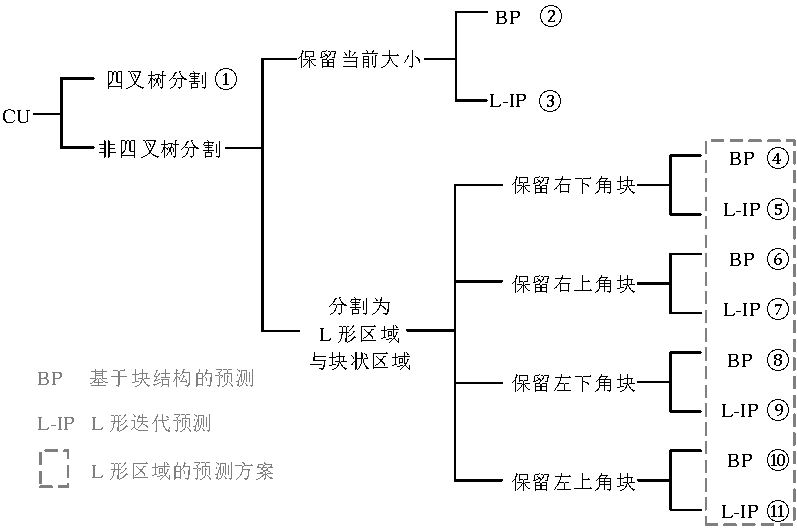
\includegraphics{L-BPIPCases.pdf}
    \caption{L-BPIP 算法 RDO 过程的比较对象}
    \label{fig:L-BPIPCases}
\end{figure}

由于存在 11 种分块可能,直接编码该信息需要 4 比特数据量。通过测试发现,四叉树分割(\ding{172})、保留右下角块 BP(\ding{174})、保留右下角块 L-IP(\ding{175})三种模式占比高达 79\%,因此决定使用变长编码编码分块模式信息,使平均码字长度最短。联合算法 L-BPIP 需要处理的另一个重要问题是编码单元的处理顺序问题。在 H.26X 框架中,由于预测过程需要使用当前编码单元右上侧和左下侧的重建点作为参考点,编码单元总是按照 Z 形扫描顺序进行处理,以保证尽可能多的参考点是已知的重建点。
L-BPIP 算法在预测过程中同时存在 L 形迭代预测和基于块结构的预测,为了保证参考点的可用性需要对编码顺序进行调整。以编码单元保留右上角块和保留右下角块为例进行说明,如图 \ref{fig:L-BPIPOrder} 所示,
\begin{figure}[hbt]
    \centering
    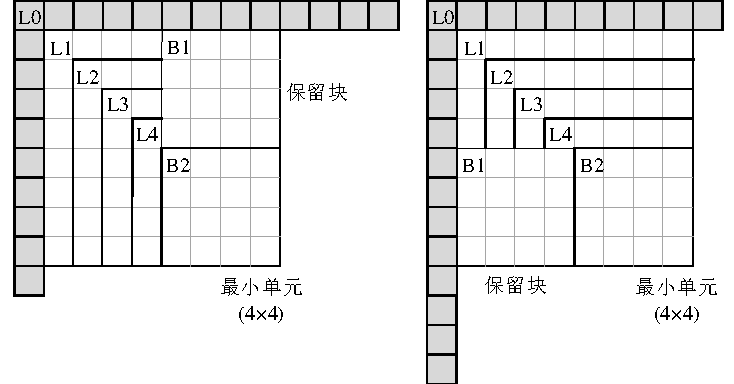
\includegraphics{L-BPIPOrder.pdf}
    \caption{L-BPIP 处理顺序说明}
    \label{fig:L-BPIPOrder}
\end{figure}
对 B2 进行预测需要 B1 边缘以及 L1\textasciitilde L4 边缘的重建点作为参考点,对 B1 进行预测需要 L1\textasciitilde L4 边缘的重建点作为参考点,对 L2\textasciitilde L4 进行预测需要其前一级 L 形区域的重建点作为参考点。
因此该编码单元最终的编码顺序为:L1$\to$L2$\to$L3$\to$L4$\to$B1$\to$B2。
在解码端将采取相同的处理顺序,可确保在对任意一个 L 形区域或块状区域进行预测时,其需要的参考点已尽可能多地被重建完成。

最后,应用 L-BPIP 算法进行实际编码测试,测试环境、测试序列、对比对象均与 \ref{cha:L-IPTest} 节所述一致,统计结果如表 \ref{tab:L-BPIPSummary} 所示。
\begin{table}[!p]
    \caption{L-BPIP 算法性能测试}
    \label{tab:L-BPIPSummary}
    \begin{minipage}{\linewidth}
        \centering
        \begin{tabular}{@{}clcccc@{}}
            \toprule
            \multirow{2}{*}{序列类别}              & \multicolumn{1}{c}{\multirow{2}{*}{序列}} & \multicolumn{4}{c}{通道}                                                                                                                                                        \\ \cmidrule(l){3-6}
                                                   & \multicolumn{1}{c}{}                      & Y                        & Cb       & Cr                  & All                                                                                                                 \\ \midrule
            \multirow{2}{*}{A}                     & PeopleOnStreet                            & -14.03\%                 & -13.86\% & -11.43\%            & -13.42\%                                                                                                            \\
                                                   & Traffic                                   & -14.30\%                 & -9.60\%  & -13.98\%            & -13.26\%                                                                                                            \\
            \multirow{5}{*}{B}                     & BasketballDrive                           & -2.74\%                  & -3.72\%  & -9.90\%             & -4.30\%                                                                                                             \\
                                                   & BQTerrace                                 & -9.32\%                  & -7.40\%  & -7.84\%             & -9.12\%                                                                                                             \\
                                                   & Cactus                                    & -3.76\%                  & -2.84\%  & -5.34\%             & -3.92\%                                                                                                             \\
                                                   & Kimono                                    & -6.74\%                  & -13.72\% & -21.14\%            & -9.07\% (-7.57\%)\footnote{圆括号中的数值为 SAP-E\upcite{SAP-SAPE,pwmResidualsPiecewiseMapping} 算法性能,作为对比} \\
                                                   & ParkScene                                 & -7.50\%                  & -9.36\%  & -10.43\%            & -7.95\% (-8.27\%)                                                                                                   \\
            \multirow{4}{*}{C}                     & BasketballDrill                           & -2.81\%                  & -2.06\%  & -4.63\%             & -3.76\%                                                                                                             \\
                                                   & BQMall                                    & -5.80\%                  & -7.06\%  & -10.91\%            & -6.55\%                                                                                                             \\
                                                   & PartyScene                                & -5.27\%                  & -6.74\%  & -8.30\%             & -5.71\%                                                                                                             \\
                                                   & RaceHorsesC                               & -8.14\%                  & -14.89\% & -15.70\%            & -9.21\%                                                                                                             \\
            \multirow{4}{*}{D}                     & BasketballPass                            & -13.02\%                 & -16.15\% & -17.76\%            & -13.79\%                                                                                                            \\
                                                   & BlowingBubbles                            & -4.89\%                  & -8.35\%  & -11.11\%            & -5.42\%                                                                                                             \\
                                                   & BQSquare                                  & -4.37\%                  & -6.20\%  & -8.33\%             & -5.05\%                                                                                                             \\
                                                   & RaceHorses                                & -8.58\%                  & -13.80\% & -14.54\%            & -9.38\%                                                                                                             \\
            \multirow{3}{*}{E}                     & FourPeople                                & -11.43\%                 & -23.62\% & -22.93\%            & -14.14\%                                                                                                            \\
                                                   & Johnny                                    & -9.15\%                  & -20.92\% & -20.63\%            & -12.29\%                                                                                                            \\
                                                   & KristenAndSara                            & -10.44\%                 & -21.16\% & -20.91\%            & -13.24\%                                                                                                            \\
            \multirow{4}{*}{F}                     & BasketballDrillText                       & -3.39\%                  & -3.30\%  & -5.83\%             & -4.50\% (-6.38\%)                                                                                                   \\
                                                   & ChinaSpeed                                & -19.37\%                 & -15.40\% & -16.22\%            & -18.56\% (-14.42\%)                                                                                                 \\
                                                   & SlideEditing                              & -16.86\%                 & -8.24\%  & -9.54\%             & -15.49\% (-11.80\%)                                                                                                 \\
                                                   & SlideShow                                 & -25.25\%                 & -26.96\% & -26.22\%            & -26.42\% (-18.92\%)                                                                                                 \\ \midrule
            \multicolumn{2}{l}{ClassA$\sim$E 均值} & -7.90\%                                   & -11.19\%                 & -13.10\% & -8.87\%                                                                                                                                   \\ \midrule
            \multicolumn{2}{l}{ClassF 均值}        & -16.22\%                                  & -13.48\%                 & -14.45\% & -16.24\% (-12.88\%)                                                                                                                       \\ \midrule
            \multicolumn{2}{l}{ClassA$\sim$F 均值} & -9.42\%                                   & -11.61\%                 & -13.35\% & -10.21\%                                                                                                                                  \\ \midrule
            \multicolumn{2}{l}{编码时间}           & \multicolumn{4}{c}{129\%}                                                                                                                                                                                                   \\ \midrule
            \multicolumn{2}{l}{解码时间}           & \multicolumn{4}{c}{103\%}                                                                                                                                                                                                   \\ \bottomrule
        \end{tabular}
    \end{minipage}
\end{table}
ClassA\textasciitilde E 中,序列 FourPeople 得到了最大的 14.14\% 的编码效率提升,均值为 8.87\%;ClassF 中,序列 SlideShow 获得了最大的 26.42\% 的编码效率提升,均值为 16.24\%。
使用编码时间衡量算法复杂度,L-BPIP 使编码时间增加了 29\%,略高于 L-IP,几乎没有影响解码时间。统计数据证明 L-BPIP 算法性能良好,具有较高的应用价值。
联合算法 L-BPIP 对比单独的 L-IP 提升了 0.89\% 的编码效率,对比 L-BP 提升了 7.87\%,证明了将二者融合的有效性和必要性。图 \ref{fig:L-BPIPVisible} 展示了联合算法对单帧图像编码块划分的显著影响,
\begin{figure}[hbt]
    \centering
    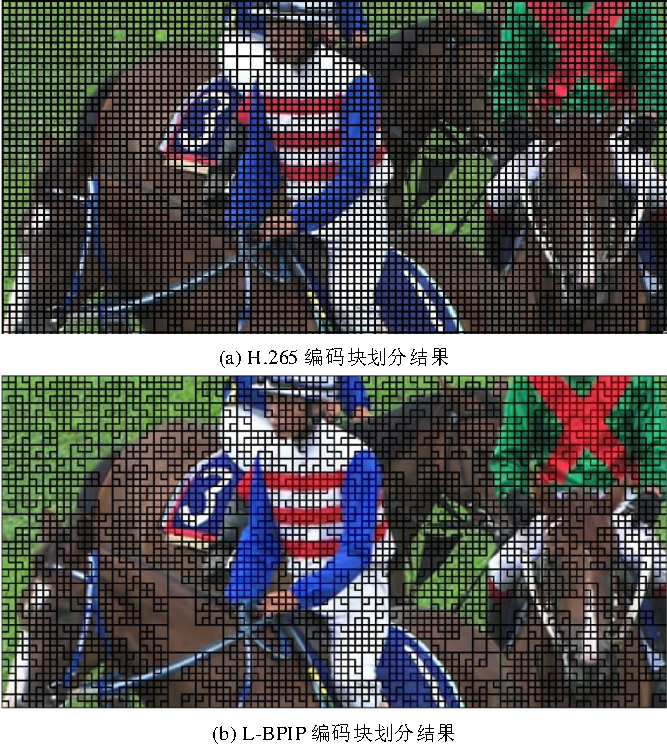
\includegraphics{L-BPIPVisible.pdf}
    \caption{H.265 标准与 L-BPIP 编码块划分结果对比}
    \label{fig:L-BPIPVisible}
\end{figure}
数据统计显示其中 16$\times$16 与 32$\times$32 的大尺寸编码块增加了 25.82\%。
很容易想象,编码块划分结果中的大尺寸块越多,所提算法发挥的性能越高,因为大尺寸块将节省大量预测模式、分块标志信息的开销,同时还能得到相同甚至更高精确度的预测结果。

此外,据我们所知,近年 H.265 无损帧内编码的优化算法中 SAP 系列得到的编码效率优化名列前茅,其中又属 SAP-E\upcite{pwmResidualsPiecewiseMapping,SAP-SAPE} 表现最为突出。因此将本课题所提算法 L-BPIP 与其进行对比,由于文献 \cite{pwmResidualsPiecewiseMapping} 中仅给出了 SAP-E 在测试序列 ParkScene(ClassB), Kimono(ClassB), BasketballDrillText(ClassF), ChinaSpeed(ClassF), SlideEditing(ClassF), SlideShow(ClassF) 的统计结果,故只对比上述 6 个序列,数据列于表 \ref{tab:L-BPIPSummary} 圆括号中。对比结果显示,在 ClassB 中,所提 L-BPIP 算法比 SAP-E 算法编码效率高 0.59\%,在 ClassF 中高 3.36\%。

\section{本章小结}
本章从软件算法层面介绍了课题提出的优化算法。对 H.26X 无损编码中帧内预测、编码块划分过程进行分析,研究其存在的缺陷。针对缺陷提出了 L-IP、L-BP、R-MED 以及 L-BPIP 共 4 个优化算法,并分别进行了测试分析,编码效率最大提高超过 10\%,证明了算法的有效性。下一章将介绍算法的硬件实现及 FPGA 原型验证系统。